\section{Theoretische Grundlagen}
\subsection{Phänomene der Supraleitung}
Im supraleitenden Zustand treten einige Phänomene auf, die bei supraleitenden Materialien nur unterhalb einer materialspezifischen kritischen Temperatur zu beobachten sind. Das ist zum Einen das Verschwinden des elektrischen Widerstands, was auch zu dieser Namensgebung geführt hat. Zum Anderen haben Supraleiter in ihrem supraleitenden Zustand ideal diamagnetisches Verhalten. Außerdem treten quantisierte magnetische Flussschläuche auf, worauf hier in diesem Kapitel aber nicht weiter eingegangen wird.

Die ersten Beobachtungen der perfekten Leitfähigkeit wurden durch die Messungen des elektrischen Widerstands der Probe gemacht, in dem der Spannungsabfall über die Probe gemessen wird. Es wurde ein Abfall des Widerstands von einem Faktor 1000 gemessen, der aber durch die Genauigkeit der Messanordnung begrenzt wurde. Mit genaueren Messaufbauten kann gesagt werden, dass der Sprung des Widerstands bei Eintritt in die Supraleitung mindestens 14 Zehnerpotenzen beträgt\cite{supraleitung}. Die herkömmlichen Modelle zur Erklärung der elektrischen Leitung können bei der Supraleitung nicht mehr angewendet werden, es zeigt sich, dass die Supraleitung ein Quanten- und Kollektivphänomen ist, worauf in Kapitel \ref{theorien} näher eingegangen wird.

Später als die perfekte Leitfähigkeit wurde der ideale Diamagnetismus durch Meißner und Ochsenfeld entdeckt. Der nach den beiden benannte Meißner-Ochsenfeld-Effekt tritt dann auf, wenn ein Permanentmagnet mit Magnetfeld, das geringer ist als ein kritisches Magnetfeld $B_c$, auf einen Supraleiter gelegt wird. Dabei werden zwei Fälle unterschieden: Zum Einen ist der Supraleiter bereits unter die kritische Temperatur $T_c$ abgekühlt und befindet sich in der supraleitenden Phase. Dann wird ein Permanentmagnet auf den Supraleiter gelegt, in dem dann durch die magnetische Flussänderung Kreisströme erzeugt werden, die ein entgegengesetztes Magnetfeld induzieren. Da der Supraleiter keinen Widerstand hat, nehmen die Ströme nicht ab, sobald der Magnet seine Gleichgewichtslage eingenommen hat. Der Permanentmagnet schwebt also, solange sich der Supraleiter unter $T_c$ befindet. Zum Anderen wird der Fall betrachtet, dass der Permanentmagnet auf den Supraleiter gelegt, wenn er sich noch oberhalb von $T_c$ befindet. Wird der Supraleiter nun unter $T_c$ abgekühlt, beginnt der Magnet beim Phasenübergang auch zu schweben. Dies kann aber nicht durch Induktion erklärt werden, da sich der magnetische Fluss nicht mehr ändert. Daher wird die Ausbildung von Abschirmströmen beim Phasenübergang zur supraleitenden Phase als Erklärung herangezogen. Dadurch wird das magnetische Feld aus dem Supraleiter bis auf in einer kleinen Schicht an der Oberfläche verdrängt. Diese Betrachtungen gelten für Supraleiter 1. Art. Bei Supraleitern 2. Art dringen die Magnetfelder teilweise in den Supraleiter ein, darauf soll aber im nächsten Kapitel \ref{arten} näher eingegangen werden.
\subsection{Supraleiter 1. und 2. Art}\label{arten}
Wie bereits gesehen, verdrängt ein Supraleiter 1. Art Magnetfelder bis zu einer bestimmten kritischen Magnetfeldstärke $B_c$ aus sich heraus. Um nicht geometrische Effekte beachten zu müssen, wird hier immer von einem langen stabförmigen Supraleiter ausgegangen. Dann kann gesagt werden, dass sich in dem Supraleiter eine Magnetisierung ausprägt, wenn ein Magnetfeld angelegt wird, das parallel zum Stab ist. Diese Magnetisierung ist proportional zur Stärke des Magnetfelds und bricht bei der kritischen Magnetfeldstärke auf $0$ zusammen. Natürlich ist diese Magnetisierung auch nur dann vorhanden, wenn sich der Supraleiter unterhalb der kritischen Temperatur $T_c$ befindet. Dies ermöglicht eine genaue Messung der kritischen Temperatur, indem die Suszeptibilität gemessen wird, die direkt von der Magnetisierung abhängt. Die kritische Magnetfeldstärke ist abhängig von der Temperatur und der kritischen Temperatur und ist empirisch gegeben durch
\begin{equation}
 B_c(T)=B_c(0)\cdot \left[1-\left(\frac{T}{T_c}\right)^2\right].
\end{equation}
\begin{figure}[htbp]  
     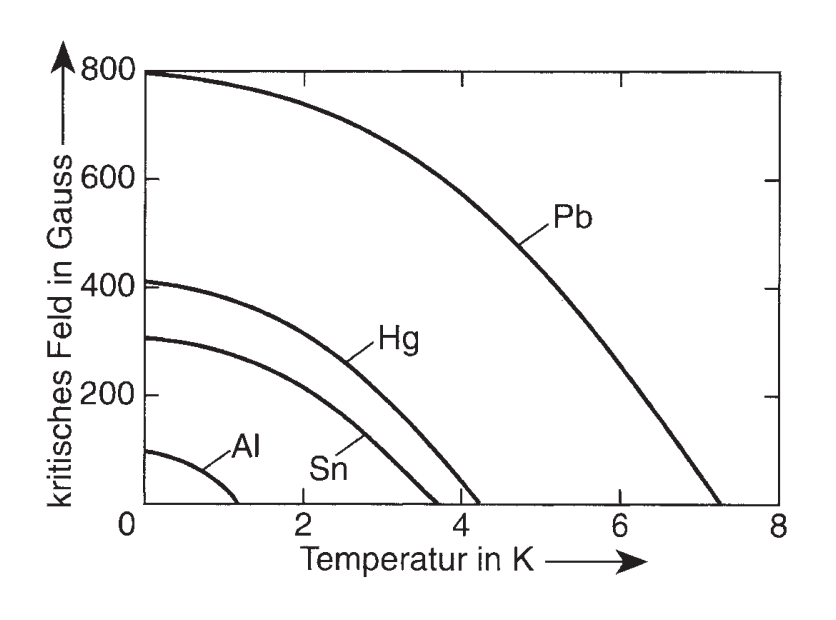
\includegraphics[width=0.99\textwidth]{1_art.png}
  \caption{Kritisches Magnetfeld in Abhängikeit der Temperatur für Al, Sn, Hg und Pb (Supraleiter 1. Art) \cite{supraleitung}}
  \label{1.art}
\end{figure}
In Abbildung \ref{1.art} erkennt man den Zusammenhang der kritischen Magnetfeldstärke mit der Temperatur des Supraleiters.

Supraleiter 2. Art verhalten sich bis zu der kritischen Magnetfeldstärke $B_{c1}$ genau wie die Supraleiter 1, sie befinden sich dort in der sogenannten Meißner-Phase. Art. oberhalb von $B_{c1}$ und unterhalb von $B_{c2}$ dringt das Magnetfeld in Form von quantisierten Flussschläuchen in den Supraleiter ein und über $B_{c2}$ verschwindet dann die Supraleitung. Schaut man sich die Magnetisierung des Supraleiters in Abhängigkeit des Magnetfeld an, wird der Unterschied zu den Supraleitern 1. Art besonders deutlich.
\begin{figure}[htbp]  
     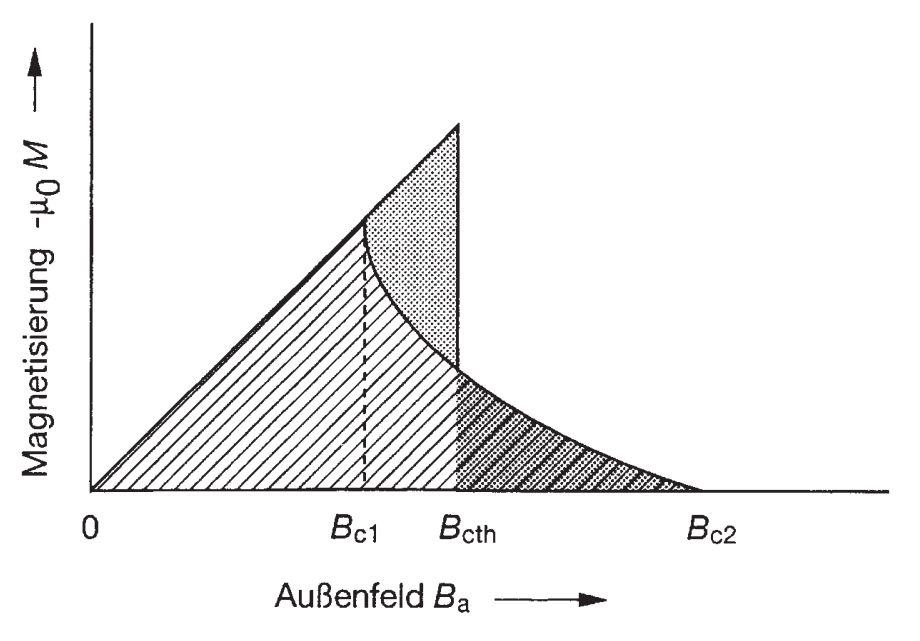
\includegraphics[width=0.99\textwidth]{2_art.png}
  \caption{Magnetisierung eines Supraleiters 2. Art, $B_{cth}$ wird so definiert, dass die punktierten Flächen gleich groß sind \cite{supraleitung}}
  \label{2.art}
\end{figure}
In Abbildung \ref{2.art} sieht man die Magnetisierung eines Supraleiters 2. Art. Dabei fällt die Magnetisierung bei $B_{c1}$ nicht wie beim Supraleiter 1. Art schlagartig auf $0$ ab, sondern nimmt monoton bis zu der kritischen Magnetfeldstärke $B_{c2}$ ab. Den Abschnitt zwischen $B_{c1}$ und $B_{c2}$ nennt man Shubnikov-Phase. Quantifiziert werden können diese Zusammenhänge mit der Ginzburg-Landau-Theorie, auf die in Kapitel \ref{ginzburg} eingegangen wird. 

Ähnlich wie beim Supraleiter 1. Art kann nun auch noch die Kurve der kritischen Magnetfeldstärken betrachtet werden (siehe Abbildung \ref{2.art2}).
\begin{figure}[htbp]  
     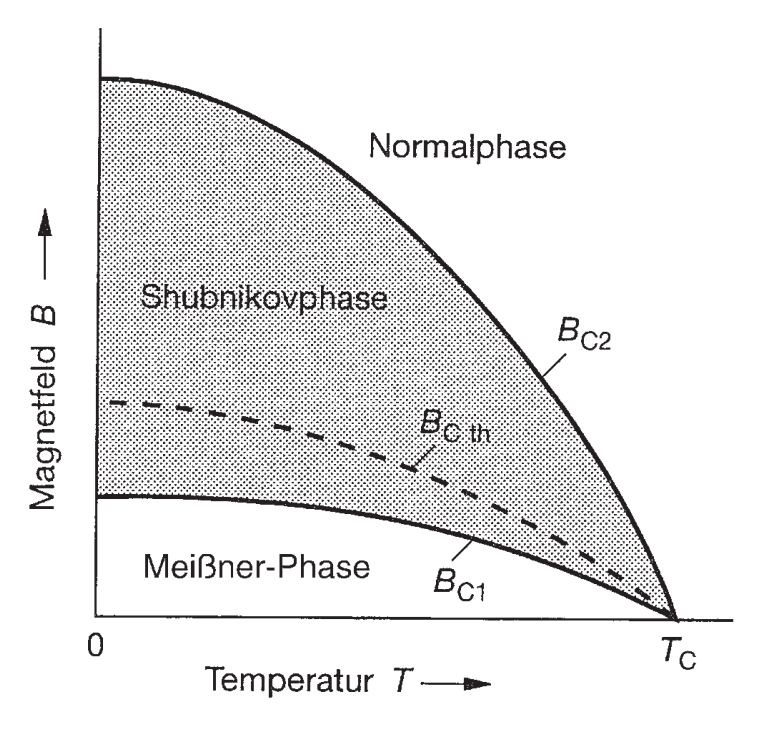
\includegraphics[width=0.68\textwidth]{2_art2.png}
  \caption{Kritische Magnetfelder in Abhängigkeit der Temperatur \cite{supraleitung}}
  \label{2.art2}
\end{figure}
Dort erkennt man, dass die Verläufe der Phasenübergangskurven ähnlich der Kurve der Supraleiter 1. Art sind, allerdings ist die kritische Magnetfeldstärke $B_{c2}$ im Allgemeinen deutlich größer als die $B_c$ bei Supraleitern 1. Art, sodass die Supraleitung bei deutlich höheren Magnetfeldern immer noch vorhanden ist. Ebenfalls erkennt man, dass alle kritischen Magnetfeldstärken bei der kritischen Temperatur $T_c$ zusammenlaufen, also dort alle kritischen Magnetfeldstärken $0$ sind.


\subsection{Theorien der Supraleitung} \label{theorien}
\subsubsection{London-Theorie}
Die London-Theorie besteht im Kern aus zwei charakteristischen Gleichungen, welche das ohmsche Gesetz für Supraleiter ersetzen. Diese beiden Gleichungen wurden von den Brüdern Fritz und Heinz London 1935 aufgestellt. Experimentell lässt sich der Verlauf des Magnetfelds innerhalb eines Supraleiters über den Meißner-Ochsenfeld-Effekt beschreiben. Aufgrund dieses sollte das Innere nämlich feldfrei sein, was sich aber experimentell nicht bestätigen lässt.

Die Brüder London postulierten folgendes Gesetz:

\begin{align}
\overrightarrow{j}=\frac{nq\hslash}{m}\overrightarrow{\nabla}S - \frac{nq^{2}}{m}\overrightarrow{A}
\end{align}

Dabei bezeichnen S die Phase der makroskopischen Wellenfunktion und A das Vektorpotential. Die beiden London-Gleichungen erhält man nun durch Umformen der Gleichung zu:

\begin{align}
\partial_t \overrightarrow{j}=\frac{nq^2}{m}\overrightarrow{E}
\end{align}

\begin{align}
rot \overrightarrow{j}=-\frac{nq^2}{m}\overrightarrow{B}
\end{align}

Mit den London-Gleichungen und den Maxwell-Gleichungen lässt sich ein exponentiell Abklingendes Magnetfeld im Inneren des Supraleiters berechnen, welches experimentell bestätigt werden kann. 


\subsubsection{Ginzburg-Landau-Theorie}\label{ginzburg}

Die Ginzburg-Landau-Theorie stellt eine makroskopische Theorie der Supraleitung über die Theorie der Phasenübergänge zweiter Ordnung dar. Gemäß dieser lässt sich die Freie Energie eines Supraleiters über einen komplexem Ordnungsparameter $\\psi$ ausdrücken:

\begin{align}
F=F_n + \alpha \vert\psi\vert^2 +\frac{\beta}{2}\vert\psi\vert^4+\frac{1}{2m*}\vert\left(\frac{\hslash}{i}\nabla +qA\right)\psi\vert^2 + \frac{\vert B \vert^2}{2\mu_0}
\end{align}

Die beiden Parameter $\alpha$ und $\beta$ sind dabei phämomenologische Parameter, welche für jedes Material neu bestimmt werden müssen. Aus der Minimierung der freien Energie kann man wiederum Gleichungen für den Ordnungsparameter und bspw. die Stromdichte herleiten, welche in enger Beziehung zu den London-Gleichungen stehen. 

Aus der Ginzburg-Landau-Theorie lassen sich zwei charakteristische Größen eines jeden Supraleiters herleiten. Diese sind erstens die Kohärenzlänge $\xi$, welche eine Größe für die Reichweite von Fluktuationen innerhalb der supraleitenden Phase ist.

\begin{align}
\xi= \sqrt{\frac{\hslash^2}{2m*\vert\alpha\vert}}
\end{align}

Weiterhin lässt sich auch die Eindringtiefe $\lambda$ des Magnetfelds in einen Supraleiter über die Ginzburg-Landau-Parameter angeben:

\begin{align}
\lambda=\sqrt{\frac{m*}{4\mu_0e^2\psi_0^2}}
\end{align}


\subsubsection{BCS-Theorie}

Die BCS-Theorie wurde 1957 von Bardeen, Cooper und Shrieffer gefunden und stellt die mikroskopische Erklärung der Supraleitung dar. Ausschlaggebend ist eine durch die Gitterschwingungen vermittelte, attraktive Wechselwirkung zwischen den Elektronen eines Kristallgitters. Diese kommt bei extrem niedrigen Temperaturen zum Tragen, da thermische Anregungen quasi nicht mehr existieren. Durch diese Wechselwirkung bilden sich aus zwei Elektronen sogenannte Cooper-Paare, welche die zweifache Elektronenmasse und -ladung aufweisen. Da hier zwei Elektronen mit Spin $\frac{1}{2}$ koppeln, besitzt das resultierende Cooper-Paar einen geradzahligen Spin und stellt damit ein Boson dar, für welches natürlich nicht mehr die Fermi-Dirac-Statistik, sondern die Bose-Einstein-Statistik gilt. Dies ist besonders ausschlaggebend für die Supraleitung, denn nun können alle gebildeten Cooper-Paare im gleichen Energiezustand vorliegen. Dieser liegt energetisch deutlich niedriger als die "normalen" Elektronenzustände, sodass im Energiespektrum eine Lücke entsteht. Stoßen die Elektronen mit Fehlstellen am Kristallgitter oder mit den Phononen der Gitterschwingungen, müssen sie Energie aufnehmen und ihren Zustand ändern. Durch die ausgebildete Energielücke ist ein Stoßen der Elektronen mit dem Kristallgitter nun jedoch nicht mehr möglich, da die bei einem Stoß aufgenommene Energie zu gering ist, um die Energielücke zu überwinden. So sind keine freien Elektronzustände vorhanden, in die die Elektronen bei einem Stoß streuen könnten. So ergibt sich die widerstandslose Bewegung der Cooper-Paare durch das Kristallgitter und damit die Supraleitung. 

Will man nun solche gebildeten Cooper-Paare wieder aufbrechen, muss dem System Energie zugefügt werden. Experimentell beobachtet man jedoch kein kontinuierliches Aufbrechen der Cooper-Paare, sondern diese sind bis zu einer bestimmten zugeführten Energie stabil. Man spricht hier von einer sogenannten Energielücke, welches das Anregungsspektrum des Supraleiters aufweist. In dieser Energielücke existieren, wie der Name schon sagt, keine Zustände für die Elektronen. Die Energie des makroskopischen Quantenzustands und damit der Cooper-Paare liegt unterhalb der Energielücke, während die "normalen" Elektronenzustände alle überhalb der Energielücke liegen. Man muss einem supraleitenden System also immer eine Mindestenergie zuführen, um die Supraleitung und die Cooper-Paare aufbrechen zu können.



